
\chapter{Описание структуры устройства}

\section{Структурная схема устройства}
\hspace{1cm}

Проектирование любого устройства начинается с определения структуры, которая описывается
его структурной схемой, которая изображена
на рисунке \ref{ris:261}.

\begin{figure}[H]
  \centering
  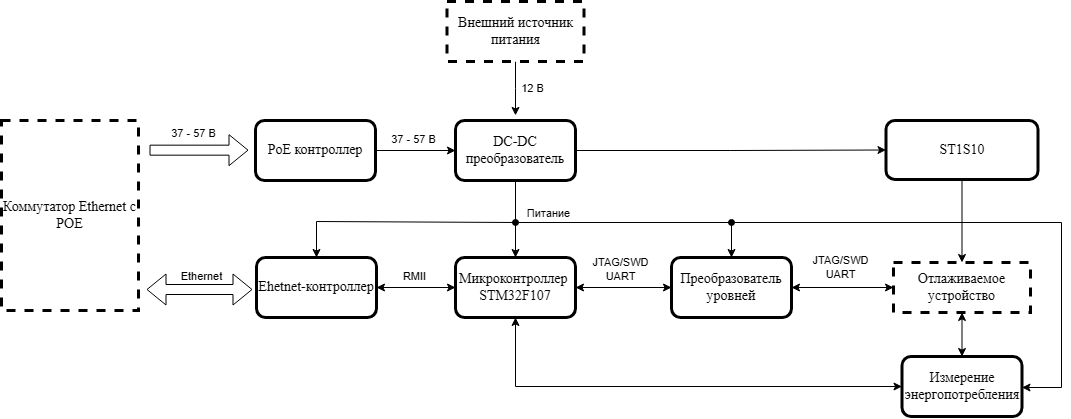
\includegraphics[scale = 0.48]{Struct Sheme.png}
  \caption{Структурная схема устройства}
  \label{ris:261}
\end{figure}

Здесь в качестве отправителя выступает условное устройство, от которого будут приходить
команды по Ethernet. PoE-контроллер, DC-DC преобразователь и регулятор ST1S10 вместе составляют 
подсистему питания,
Ethernet-контроллер является подсистемой Ethernet, STM32F107 -- подсистема управления, 
преобразователь уровней является подсистемой преобразования уровней, измерение энергопотребления --
это одноименная подсистема, а отлаживаемое устройство представляет собой целевой микроконтроллер,
на который будет отправляться прошивка и чье энергопотребление будет измеряться.

\section{Подсистема управления}
\hspace{1cm} 

Главным компонентом любого устройства является его подсистема управления.

В качестве микроконтроллера было решено использовать
STM32F107VCT6 из-за его следующих преимуществ \cite{STM32:datasheet}:

\begin{itemize}
    \item \textit{Хорошо проработанная документация} -- компания
     STMicroelectronics является одним из лидеров на рынке микроконтроллеров, во многом благодаря
     замечательной документации, которая позволяет создавать на базе их решений проработанные
     и, по большей части, предсказуемо работающие проекты. Важно быть уверенным, что при разработке
     устройства микроконтроллер не начнет показывать <<недокументированные>> возможности и
     различные баги, и репутация компании STMicroelectronics позволяет быть в этом
     уверенным. Антипримером может служить компания Espressif, чьи многочисленные ошибки,
     выявленные после выпуска очередного микроконтроллера, иногда выливаются в довольно
     объемные errata документы.
    \item \textit{Библиотеки} -- наличие удобных и, самое главное, пригодных в использовании 
     библиотек позолит значительно ускорить время разработки. Для микроконтроллеров
     компании STM32 написано большое количество популярных библиотек, таких
     как HAL, LL, CMSIS, libopencm3 и другие.
    \item \textit{Большое количество готовых решений} -- некоторые из функций разрабатываемой
     системы могли быть реализованы ранее индивидуальным разработчиком, 
     сообществом или предприятием. Разработку всегда стоит начинать с поиска готовых или похожих 
     решений, которые, возможно, уже были разработаны и ждут интеграции в проект. Используемое
     в STM32F107VCT6 ядро сильно повышает шансы найти что-то готовое или то, что сильно 
     ускорит и упростит разработку устройства, позволяя не писать отдельные модули с <<нуля>>.
     \cite{Lakamera:embed}. Рамках разработки отладчика мы будем использовать решения из проектов 
     Blackmagick и Energymon, благо, что их лицензии позволяют использовать их исходный код.
    \item \textit{Доступность} -- в <<санкционную>> эпоху доступность компонента может стать 
     решающим фактором при выборе. Благодаря своей массовости микроконтроллеры серии STM32 
     можно легко найти как у дистрибьюторов ориентированных на крупные компании, так и на тех,
     кто работает с физическими лицами, что важно в рамках студенческой дипломной работы.
\end{itemize}

\section{Подсистема питания}
\hspace{1cm} 

Невозможно представить устройство без подсистемы питания, которая является его <<сердцем>>,
обеспечивая электроэнергией все остальные подсистемы. Плохо спроектированная система питания
может стать большой проблемой, вплоть до вывода из строя отдельной подсистемы или устройства
в целом.

В качестве питания для отладчика была выбрана связка из PoE + DC-DC преобразователь, 
выполненный по технологии изолированный fly-buck, с возможностью подключения внешнего питания. 

PoE (Power over Ethernet) — это технология передачи удаленным Ethernet-устройствам по 
витой паре электропитания вместе с данными. Данная технология позволяет питать подключенные 
устройства, к которым невозможно или нежелательно проводить кабели для питания.

Технология PoE была выбрана по причине  удобства её использования в устройствах с передачей
данных по Ethernet. Это избавляет от необходимости подключения дополнительных проводов, что
делает отладчик более мобильным. С другой стороны необходимо сохранить возможность подключения
питания более традиционными способами, например через внешний блок питания.

Характеристики различных стандартов PoE представлены в таблице \ref{PoE}.

\begin{table}[H]
    \caption{Основные характеристики стандартов PoE} 
    \label{PoE}
    \begin{center}
    \begin{tabular}{|c|p{2cm}|p{2cm}|p{2cm}|p{2cm}|}
    \hline
  Характеристика/Стандарт & 802.3af  &  802.3at   & 802.3bt & 802.3bt \\ \hline
    Выходная мощность, Вт & 15,4  & 30 А & 60 &  90 \\ \hline
    Мощность на устройстве, Вт & 12,95 & 25,5 & 51 & 71,3  \\ \hline
    Выходное напряжение на источнике, В & 44--57 & 50--57 & 50--57 & 52--57 \\ \hline
    Напряжение на приемнике, В & 37--57 & 42,5--57 & 42,5--57 & 41,1--57  \\ \hline
    Максимальный ток в витой паре, мА & 350 & 600 & 600 & 960  \\ \hline
    \end{tabular}
    \end{center}
\end{table} 

Так же стоит упомянуть наименее стандартизированный Passive PoE, которой может поддерживать только 
электрические характеристики соответствия стандарту 802.3af, но не протокольные. Passive PoE не 
совместим со стандартом IEEE 802.3af. Passive PoE не опрашивает питаемое устройство и не согласовывает
мощность. По свободным проводникам витой пары просто подается постоянное напряжение. Поэтому, 
если соединить источник PoE и потребитель, несовместимые друг с другом, оборудование может сгореть: 
сразу или через некоторое время, в результате постоянного перегрева и подгорания плат 
\cite{DeterminationPoE}.

Для понимания какой стандарт PoE будет необходимо реализовать в отладчике
можно оценочно проанализировать энергопотребление самых энергозатратных элементов устройства.

Максимальная потребляемая мощность микроконтроллера STM32F107VCT6 в корпусе LQFP64 составляет 
444 мВт \cite{STM32:datasheet}, ток потребления выбранного контроллера PoE до 50 мА 
\cite{TPS2376:datasheet}, усредненный ток потребления измерительного операционного усилителя --
до 5 мА, потребляемая мощность выбранной PHY микросхемы до 270 мВт \cite{DP83848:datasheet}. Так же
планируемая мощность потребления отлаживаемого устройства равна 5 Вт.
С учетом усредненного КПД импульсного DC-DC преобразователя, который составляет 70 \%, можно
рассчитывать на то, что мощности 12,95 Вт, которую обеспечивает стандарт 802.3af, должно хватить 
\cite{IEEE 802.3af}.

Для маломощных источников питания часто используют fly-buck-конверторы, они же обратноходовые
преобразователи. Преимуществами данного решения являются \cite{PowerElectronic:FlyBack}:
\begin{itemize}
  \item Сравнительная простота реализации
  \item Малое количество используемых элементов
  \item Дешевизна
  \item Малая чувствительность к короткому замыканию на выходе
\end{itemize}

Использование же изолированного fly-back преобразователя дает гальваническую развязку по питанию,
что защищает пользователя в случаях случайного касания разъемов, к которым в отладчике 
планируются свободный доступ.

\section{Подсистема измерения энергопотребления}
\hspace{1cm} 

Для измерения тока используется метод снятия напряжения с шунта,
 который представляет собой резистор известного сопротивления с малым отклонением номинала,
 который обычно составляет менее 1\%, с помощью операционного
усилителя, включенного по схеме дифференциального усилителя.
Существует два основных способа подключения измерительной цепи – со стороны никого
или высокого уровня. В ходе производственной практики были рассмотрены и изучены схемы
подключения измерительной цепи по смехе верхнего плеча, которая представлена на рисунке
\ref{ris:231} и по схеме нижнего плеча, которая представлена на рисунке \ref{ris:232} 
\cite{CurrentMeasSolution}.


\begin{figure}[H]
  \centering
  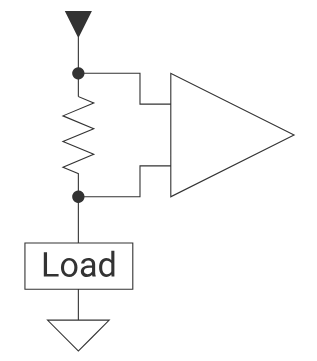
\includegraphics[scale = 0.65]{Hihg-side Meas.png}
  \caption{Схема верхнего плеча}
  \label{ris:231}
\end{figure}

\begin{figure}[H]
  \centering
  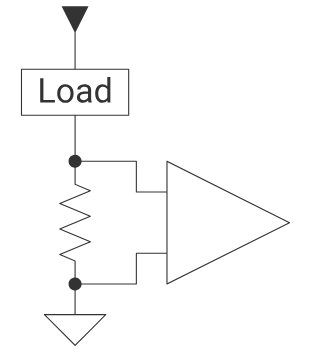
\includegraphics[scale = 0.65]{Low-side Meas.png}
  \caption{Схема нижнего плеча}
  \label{ris:232}
\end{figure}

Измерение тока в конфигурации нижнего плеча заключается в размещении измерительного 
элемента между нагрузкой и землей. Этот тип решения довольно легко реализовать, поскольку 
напряжение на измерительном элементе измеряется по отношению к массе цепи. Усилитель 
работает с низкими значениями напряжения (порядка милливольт по отношению к массе схемы), 
что значительно упрощает подбор компонентов и снижает его стоимость.

В случае работы с малыми сигналами довольно большую роль играет входное напряжение 
смещения усилителя. Чем меньше значение этого параметра, тем выше точность измерения.

Несмотря на эти недостатки, измерение тока на стороне низкого напряжения является хорошим выбором,
когда нагрузку не нужно подключать напрямую к земле и где нет необходимости обнаруживать 
короткие замыкания на массу. Но в случае устройств, которые должны соответствовать 
более строгим требованиям безопасности, измерение тока на стороне высокого 
напряжения является лучшим выбором.
После усиления напряжение на выходе ОУ оцифровывается 12-битным АЦП с опорным 
напряжением 3,3 В, соответственно, каждый значащий разряд АЦП -- это 3,3/4096 = 0,805 мВ.
При коэффициенте усиления Ку = 50 нашего ОУ, шаг измеряемого напряжения
на шунте -- около 16 мкВ. Соответственно, при шунтах 100, 1 и 0,01 Ом младшему 
разряду АЦП соответствует потребляемый ток в 0,16 мкА, 16 мкА и 1,6 мА соответственно 
\cite{GooglePatent:1}.

Так же подсистема измерения токопотребления включает в себя переключаемые шунты, принцип работы которых 
представлен на рисунке \ref{ris:ShuntSwitching} \cite{GooglePatent:2}.

\begin{figure}[H]
  \centering
  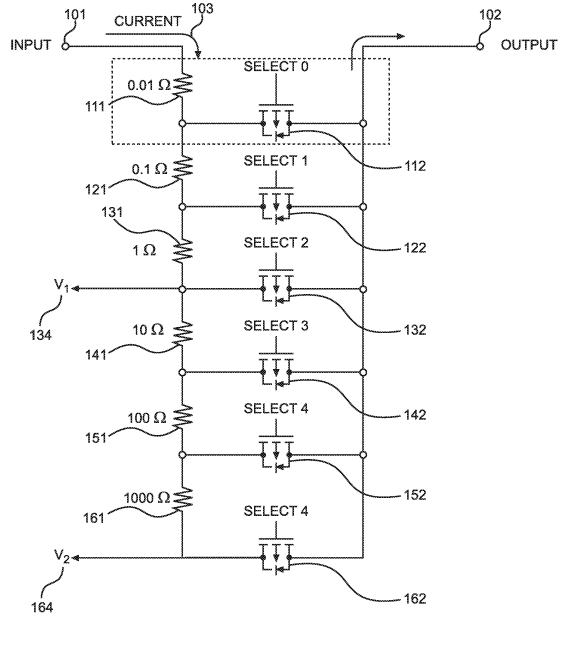
\includegraphics[scale = 0.6]{ShuntSwitching.png}
  \caption{Схема переключения шунтов}
  \label{ris:ShuntSwitching}
\end{figure}

На данном рисунке показан путь протекания тока через определенные шунты, которые, в зависимости от 
открытого транзистора, включаются или исключаются из пути прохождения тока. 



\section{Подсистема преобразования уровней}
\hspace{1cm}

Подсистема преобразования уровней нужна для согласования уровней и изоляции от паразитного 
питания шин с разным напряжением. Подсистема будет согласовывать уровни напряжения между
отладчиком и отлаживаем устройством по линиям передачи данных. 

Надежным и быстрым решением будет использование специализированной микросхемы 74LVC2T45, из-за
следующих преимуществ \cite{SN74LVC2T45:datasheet}:
\begin{itemize}
  \item Работает во всем диапазоне напряжений от 1,65 В до 5,5 В
  \item Имеет функцию изоляции напряжения питания отлаживаемого устройства переводом каналов в
  высокоимпедансное состояние
  \item Малый ток потребления -- до 4 мкА
  \item Максимальная скорость передачи данных 75 Мбит/с
  \item Имеет защиту от статики в соответствии со стандартом JESD20
  \item Есть возможность переключения направления, что особенно важно при работе с отладочным 
  интерфейсом SWD.
\end{itemize}
 Ее функциональная диаграмма изображена на рисунке \ref{ris:241}.

\begin{figure}[H]
  \centering
  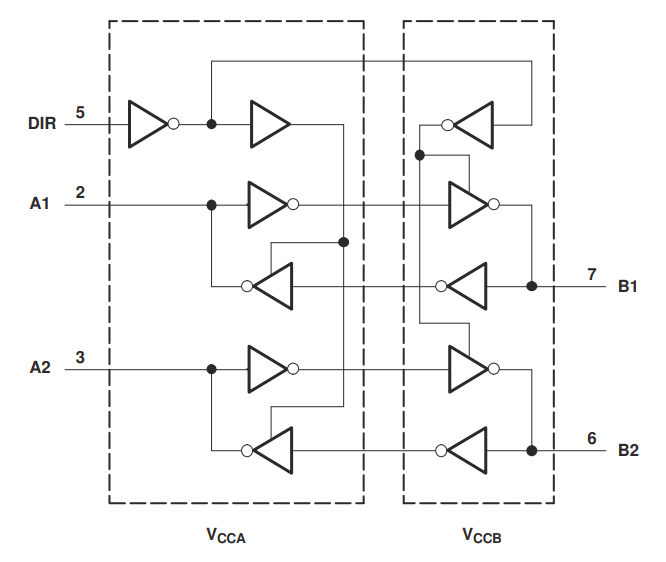
\includegraphics[scale = 0.75]{ris241.png}
  \caption{Функциональная схема 74LVC2T45}
  \label{ris:241}
\end{figure}


\section{Подсистема Ethernet}
\hspace{1cm}

Данная подсистема будет состоять из входного бестрансформаторного разъема типа RJ-45, 
согласующего трансформатора, и PHY-микросхемы, предназначенной для выполнения функций 
физического уровня сетевой модели OSI.

Связка из бестрансформаторного разъема и согласующего трансформатора отдельной
микросхемой была выбрана для совместимости с PoE, так как большинство доступных разъемов со 
встроенным трансформатором не имеют отводов от средней точки трансформатора со стороны кабеля,
что необходимо для работы PoE. 

На рисунке \ref{ris:251} изображена внутренняя структура согласующего трансформатора на примере микросхемы
HX1188NL. Проблема у большинства разъемов со встроенным трансформатором возникала из-за
отсутствия связей 2 и 7. 

\begin{figure}[H]
  \centering
  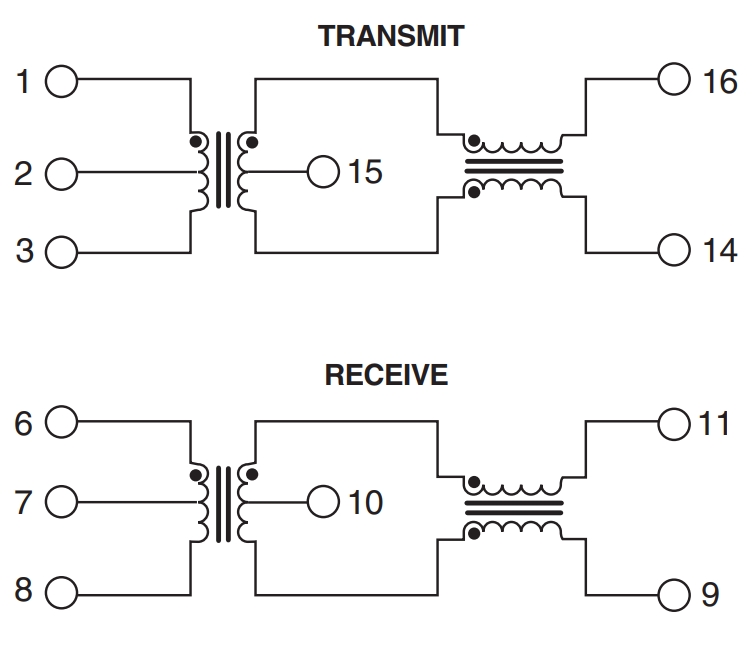
\includegraphics[scale = 0.75]{ris251.png}
  \caption{Внутренняя структура HX1188NL}
  \label{ris:251}
\end{figure}

В качестве Ethernet-контроллера была выбрана микросхема DP83848 \cite{DP83848:datasheet} из-за того, 
что при отладке прошивки использовалась отладочная плата именно с этой PHY-микросхемой <<на борту>>. 
Использование другой микросхемы привело бы к увлечению времени отладки устройства и более глубокой 
переработки уже готового решения, что нерационально.



%В случае нехватки объема добавить разгон про модель OSI

